\pattern{Publish and Subscribe}
\begin{summary}
    Allows publishers (senders) to broadcast messages to several subscribers
    (receivers) without them being tightly coupled. Essentially, the publishers
    are unaware of which application is going to receive the message whereas
    the subscribers do not really care about who actually sent it.
\end{summary}


\subsubsection{Implementation}
\begin{description}
    \item[Publisher] Application that sends messages. 

    \item[Broker] Delivers every message sent to all suitable subscribers.
        Publishers send messages the broker, and the subscribers allow the
        broker to filter the messages. The broker then routes messages to the
        subscribers that have subscribed to the particular topic.

    \item[Subscriber] Applications that receive messages. When publishers push
        messages not all subscribers receive them. A filtering
        process only delivers messages to interested subscribers. There are two
        primary methods of filtering messages: topic-based and content-based
        filtering systems.

    \item[Topic-based filtering] Messages are broadcasted into logical channels
        or topics. This system allows subscribes to only receive messages that
        they have subscribed to. All subscribers that are subscribed to a
        particular topic will receive all of the same messages.

    \item[Content-based filtering] Messages are only delivered to a subscriber
        if the content matches the constraints that are defined and set by the
        subscriber. 
\end{description}

The publish-subscribe architecture style is resilient to many changes. Adding
or removing topics is convenient and scalable because it can be done without
changing the architecture.

\comparison{\begin{itemize}
        \item Low coupling: Publishers and subscribers are different entities,
            allowing them to function without being aware of each other.

        \item Reliability: If any of the publishers and/or subscribers stop
            working, this will not impact other publishers or subscribers and
            the application may still be fully functional.

        \item Scalability: There are several flavours of communication styles
            that the Pub-Sub model supports, from 1-to-1, to many-to-many. All
            of these communication styles are possible due to how loosely
            coupled the components are.

        \item Scalability: Publishers and subscribers to be added and removed
            dynamically, as each topic can have any number of publishers and
            subscribers. Therefore, scaling in terms of adding multiple
            publishers and subscribers can be easily done.

    \end{itemize}
}{\begin{itemize}
        \item Stability: Publishers do not directly communicate and do not
            have complete knowledge of their subscribers. As a result,
            publishers cannot guarantee that messages have been properly
            delivered to their subscribers. The message delivering process is
            dependent on the broker properly delivering the messages. The model
            can be modified to increase stability by having subscribers sending
            a confirmation receipt back to publishers, however this adds
            another level of complexity.
        \item High Semantic Coupling: After the data structure for a message is
            created, modifying this existing message type and/or format can get
            very difficult. All publishers and subscribers that use the message
            type must be altered to accept the new message type. From a
            developer’s standpoint, this may be impossible to do if the
            publisher or subscriber is in an external API.
\end{itemize}}

\begin{nfps}
\item[Scalability] Scalability is supported by Pub-Sub. As stated in the
    advantages section of this document, due to the low coupling nature of this
    architecture adding more publishers and subscribers can be done very
    efficiently which can help scaling applications a lot.
\item[Dependability] There are aspects of dependability that are inhibited by
    Pub-Sub. This relates to the stability disadvantage of Pub-Sub, as the
    publisher has no guarantees of messages being delivered. Thus, the
    guarantee of dependability is sacrificed.
\item[Adaptability] Similar to the advantages section of this document, adding
    new features such as subscribers, publishers and topics can be done easily.
    However, as discussed in the disadvantages section, modifying existing
    messages types can get harder.
\end{nfps}

\begin{center}
    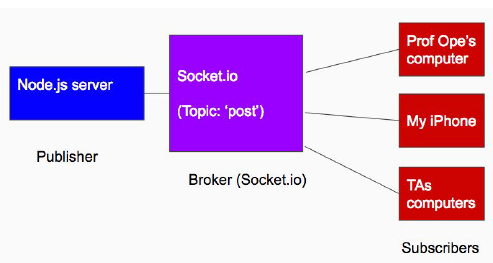
\includegraphics[width=0.4\textwidth]{./pub-sub1}
    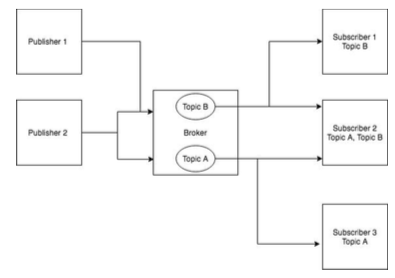
\includegraphics[width=0.4\textwidth]{./pub-sub2}
\end{center}
